\documentclass[twoside]{book}

% Packages required by doxygen
\usepackage{fixltx2e}
\usepackage{calc}
\usepackage{doxygen}
\usepackage[export]{adjustbox} % also loads graphicx
\usepackage{graphicx}
\usepackage[utf8]{inputenc}
\usepackage{makeidx}
\usepackage{multicol}
\usepackage{multirow}
\PassOptionsToPackage{warn}{textcomp}
\usepackage{textcomp}
\usepackage[nointegrals]{wasysym}
\usepackage[table]{xcolor}

% Font selection
\usepackage[T1]{fontenc}
\usepackage[scaled=.90]{helvet}
\usepackage{courier}
\usepackage{amssymb}
\usepackage{sectsty}
\renewcommand{\familydefault}{\sfdefault}
\allsectionsfont{%
  \fontseries{bc}\selectfont%
  \color{darkgray}%
}
\renewcommand{\DoxyLabelFont}{%
  \fontseries{bc}\selectfont%
  \color{darkgray}%
}
\newcommand{\+}{\discretionary{\mbox{\scriptsize$\hookleftarrow$}}{}{}}

% Page & text layout
\usepackage{geometry}
\geometry{%
  a4paper,%
  top=2.5cm,%
  bottom=2.5cm,%
  left=2.5cm,%
  right=2.5cm%
}
\tolerance=750
\hfuzz=15pt
\hbadness=750
\setlength{\emergencystretch}{15pt}
\setlength{\parindent}{0cm}
\setlength{\parskip}{3ex plus 2ex minus 2ex}
\makeatletter
\renewcommand{\paragraph}{%
  \@startsection{paragraph}{4}{0ex}{-1.0ex}{1.0ex}{%
    \normalfont\normalsize\bfseries\SS@parafont%
  }%
}
\renewcommand{\subparagraph}{%
  \@startsection{subparagraph}{5}{0ex}{-1.0ex}{1.0ex}{%
    \normalfont\normalsize\bfseries\SS@subparafont%
  }%
}
\makeatother

% Headers & footers
\usepackage{fancyhdr}
\pagestyle{fancyplain}
\fancyhead[LE]{\fancyplain{}{\bfseries\thepage}}
\fancyhead[CE]{\fancyplain{}{}}
\fancyhead[RE]{\fancyplain{}{\bfseries\leftmark}}
\fancyhead[LO]{\fancyplain{}{\bfseries\rightmark}}
\fancyhead[CO]{\fancyplain{}{}}
\fancyhead[RO]{\fancyplain{}{\bfseries\thepage}}
\fancyfoot[LE]{\fancyplain{}{}}
\fancyfoot[CE]{\fancyplain{}{}}
\fancyfoot[RE]{\fancyplain{}{\bfseries\scriptsize Generated by Doxygen }}
\fancyfoot[LO]{\fancyplain{}{\bfseries\scriptsize Generated by Doxygen }}
\fancyfoot[CO]{\fancyplain{}{}}
\fancyfoot[RO]{\fancyplain{}{}}
\renewcommand{\footrulewidth}{0.4pt}
\renewcommand{\chaptermark}[1]{%
  \markboth{#1}{}%
}
\renewcommand{\sectionmark}[1]{%
  \markright{\thesection\ #1}%
}

% Indices & bibliography
\usepackage{natbib}
\usepackage[titles]{tocloft}
\setcounter{tocdepth}{3}
\setcounter{secnumdepth}{5}
\makeindex

% Hyperlinks (required, but should be loaded last)
\usepackage{ifpdf}
\ifpdf
  \usepackage[pdftex,pagebackref=true]{hyperref}
\else
  \usepackage[ps2pdf,pagebackref=true]{hyperref}
\fi
\hypersetup{%
  colorlinks=true,%
  linkcolor=blue,%
  citecolor=blue,%
  unicode%
}

% Custom commands
\newcommand{\clearemptydoublepage}{%
  \newpage{\pagestyle{empty}\cleardoublepage}%
}

\usepackage{caption}
\captionsetup{labelsep=space,justification=centering,font={bf},singlelinecheck=off,skip=4pt,position=top}

%===== C O N T E N T S =====

\begin{document}

% Titlepage & ToC
\hypersetup{pageanchor=false,
             bookmarksnumbered=true,
             pdfencoding=unicode
            }
\pagenumbering{alph}
\begin{titlepage}
\vspace*{7cm}
\begin{center}%
{\Large F\+F\+Neural\+Net }\\
\vspace*{1cm}
{\large Generated by Doxygen 1.8.14}\\
\end{center}
\end{titlepage}
\clearemptydoublepage
\pagenumbering{roman}
\tableofcontents
\clearemptydoublepage
\pagenumbering{arabic}
\hypersetup{pageanchor=true}

%--- Begin generated contents ---
\chapter{Hierarchical Index}
\section{Class Hierarchy}
This inheritance list is sorted roughly, but not completely, alphabetically\+:\begin{DoxyCompactList}
\item \contentsline{section}{Act\+Fun\+Test}{\pageref{class_act_fun_test}}{}
\item \contentsline{section}{F\+F\+Neural\+Net}{\pageref{class_f_f_neural_net}}{}
\item \contentsline{section}{F\+F\+N\+N\+Test}{\pageref{class_f_f_n_n_test}}{}
\item \contentsline{section}{M\+N\+I\+S\+T\+File\+Parser}{\pageref{class_m_n_i_s_t_file_parser}}{}
\begin{DoxyCompactList}
\item \contentsline{section}{Image\+Parser}{\pageref{class_image_parser}}{}
\item \contentsline{section}{Label\+Parser}{\pageref{class_label_parser}}{}
\end{DoxyCompactList}
\end{DoxyCompactList}

\chapter{Class Index}
\section{Class List}
Here are the classes, structs, unions and interfaces with brief descriptions\+:\begin{DoxyCompactList}
\item\contentsline{section}{\mbox{\hyperlink{class_act_fun_test}{Act\+Fun\+Test}} }{\pageref{class_act_fun_test}}{}
\item\contentsline{section}{\mbox{\hyperlink{class_f_f_neural_net}{F\+F\+Neural\+Net}} \\*Simple feed-\/forward network with single activation function at all levels }{\pageref{class_f_f_neural_net}}{}
\item\contentsline{section}{\mbox{\hyperlink{class_f_f_n_n_test}{F\+F\+N\+N\+Test}} }{\pageref{class_f_f_n_n_test}}{}
\item\contentsline{section}{\mbox{\hyperlink{class_image_parser}{Image\+Parser}} }{\pageref{class_image_parser}}{}
\item\contentsline{section}{\mbox{\hyperlink{class_label_parser}{Label\+Parser}} }{\pageref{class_label_parser}}{}
\item\contentsline{section}{\mbox{\hyperlink{class_m_n_i_s_t_file_parser}{M\+N\+I\+S\+T\+File\+Parser}} }{\pageref{class_m_n_i_s_t_file_parser}}{}
\end{DoxyCompactList}

\chapter{Class Documentation}
\hypertarget{class_act_fun_test}{}\section{Act\+Fun\+Test Class Reference}
\label{class_act_fun_test}\index{Act\+Fun\+Test@{Act\+Fun\+Test}}
\subsection*{Public Member Functions}
\begin{DoxyCompactItemize}
\item 
\mbox{\Hypertarget{class_act_fun_test_a378665ab0f64d897717b5e6b28aa4afa}\label{class_act_fun_test_a378665ab0f64d897717b5e6b28aa4afa}} 
void {\bfseries Run\+Tests} (void)
\item 
\mbox{\Hypertarget{class_act_fun_test_a0ae20979fb12ac63bf7b5441bb05094a}\label{class_act_fun_test_a0ae20979fb12ac63bf7b5441bb05094a}} 
bool {\bfseries run\+Re\+L\+U\+Test} (void)
\item 
\mbox{\Hypertarget{class_act_fun_test_a377bbed6666f6f9d5179e301fbf2f569}\label{class_act_fun_test_a377bbed6666f6f9d5179e301fbf2f569}} 
bool {\bfseries run\+Sigmoid\+Test} (void)
\item 
\mbox{\Hypertarget{class_act_fun_test_a596cae9fffae945ad0f7ef172bbe80f5}\label{class_act_fun_test_a596cae9fffae945ad0f7ef172bbe80f5}} 
bool {\bfseries xany} (std\+::vector$<$ bool $>$)
\end{DoxyCompactItemize}


The documentation for this class was generated from the following files\+:\begin{DoxyCompactItemize}
\item 
C\+:/\+Users/charc/source/repos/ff\+Neural\+Net/\+Neural\+Net/Act\+Fun\+Test.\+h\item 
C\+:/\+Users/charc/source/repos/ff\+Neural\+Net/\+Neural\+Net/Act\+Fun\+Test.\+cpp\end{DoxyCompactItemize}

\hypertarget{class_f_f_neural_net}{}\section{F\+F\+Neural\+Net Class Reference}
\label{class_f_f_neural_net}\index{F\+F\+Neural\+Net@{F\+F\+Neural\+Net}}


Simple feed-\/forward network with single activation function at all levels.  




{\ttfamily \#include $<$F\+F\+Neural\+Net.\+h$>$}

\subsection*{Public Member Functions}
\begin{DoxyCompactItemize}
\item 
\mbox{\Hypertarget{class_f_f_neural_net_a51b79470c6d19c7b7d37f043c695b5b0}\label{class_f_f_neural_net_a51b79470c6d19c7b7d37f043c695b5b0}} 
{\bfseries F\+F\+Neural\+Net} (int n\+Input\+Nodes=1, int n\+Hidden\+Nodes=1, int n\+Hidden\+Layers=1, int n\+Output\+Nodes=1, double rate=0.\+2, std\+::pair$<$ std\+::function$<$ Eigen\+::\+Matrix\+Xd(Eigen\+::\+Matrix\+Xd)$>$, std\+::function$<$ Eigen\+::\+Matrix\+Xd(Eigen\+::\+Matrix\+Xd)$>$$>$ A\+C\+T\+F\+UN=std\+::pair$<$ std\+::function$<$ Eigen\+::\+Matrix\+Xd(Eigen\+::\+Matrix\+Xd)$>$, std\+::function$<$ Eigen\+::\+Matrix\+Xd(Eigen\+::\+Matrix\+Xd)$>$$>$(act\+Funs\+::sigmoid, act\+Funs\+::sigmoid\+\_\+prime))
\item 
\mbox{\Hypertarget{class_f_f_neural_net_ac419314557a65bebfa9d457673cc2211}\label{class_f_f_neural_net_ac419314557a65bebfa9d457673cc2211}} 
void {\bfseries train} (Eigen\+::\+Matrix\+Xd $\ast$X, Eigen\+::\+Matrix\+Xd $\ast$Y, double tol)
\item 
\mbox{\Hypertarget{class_f_f_neural_net_ab8d26640e55c0422527822124c4216b7}\label{class_f_f_neural_net_ab8d26640e55c0422527822124c4216b7}} 
double {\bfseries test} (Eigen\+::\+Matrix\+Xd $\ast$X, Eigen\+::\+Matrix\+Xd $\ast$Y)
\item 
\mbox{\Hypertarget{class_f_f_neural_net_ad42d220ba8a00ede1f60f6674eecc69a}\label{class_f_f_neural_net_ad42d220ba8a00ede1f60f6674eecc69a}} 
Eigen\+::\+Matrix\+Xd {\bfseries predict} (Eigen\+::\+Matrix\+Xd)
\end{DoxyCompactItemize}
\subsection*{Friends}
\begin{DoxyCompactItemize}
\item 
\mbox{\Hypertarget{class_f_f_neural_net_a63fe7da00177d41882169c5f904d5652}\label{class_f_f_neural_net_a63fe7da00177d41882169c5f904d5652}} 
class {\bfseries F\+F\+N\+N\+Test}
\end{DoxyCompactItemize}


\subsection{Detailed Description}
Simple feed-\/forward network with single activation function at all levels. 

The documentation for this class was generated from the following files\+:\begin{DoxyCompactItemize}
\item 
C\+:/\+Users/charc/source/repos/ff\+Neural\+Net/\+Neural\+Net/F\+F\+Neural\+Net.\+h\item 
C\+:/\+Users/charc/source/repos/ff\+Neural\+Net/\+Neural\+Net/F\+F\+Neural\+Net.\+cpp\end{DoxyCompactItemize}

\hypertarget{class_f_f_n_n_test}{}\section{F\+F\+N\+N\+Test Class Reference}
\label{class_f_f_n_n_test}\index{F\+F\+N\+N\+Test@{F\+F\+N\+N\+Test}}
\subsection*{Public Member Functions}
\begin{DoxyCompactItemize}
\item 
\mbox{\Hypertarget{class_f_f_n_n_test_a098a5e288baa36728d016d655dd8a13b}\label{class_f_f_n_n_test_a098a5e288baa36728d016d655dd8a13b}} 
void {\bfseries Run\+Tests} (void)
\item 
\mbox{\Hypertarget{class_f_f_n_n_test_a8d7a4ff5daf1abe41d8aa3263dac1073}\label{class_f_f_n_n_test_a8d7a4ff5daf1abe41d8aa3263dac1073}} 
bool {\bfseries xany} (std\+::vector$<$ bool $>$ a)
\item 
\mbox{\Hypertarget{class_f_f_n_n_test_a83c05957353b5bb0d9204c110234a9ef}\label{class_f_f_n_n_test_a83c05957353b5bb0d9204c110234a9ef}} 
bool {\bfseries test\+Not} (void)
\item 
\mbox{\Hypertarget{class_f_f_n_n_test_a65f08161ecda5b43099837bf04885fbd}\label{class_f_f_n_n_test_a65f08161ecda5b43099837bf04885fbd}} 
bool {\bfseries test\+Id\+Regression} (void)
\item 
\mbox{\Hypertarget{class_f_f_n_n_test_a0cc662c87158796a4114a01aa3badee9}\label{class_f_f_n_n_test_a0cc662c87158796a4114a01aa3badee9}} 
bool {\bfseries test\+M\+N\+I\+ST} (int train\+\_\+record\+\_\+cap=-\/1, int test\+\_\+record\+\_\+cap=-\/1)
\end{DoxyCompactItemize}


The documentation for this class was generated from the following files\+:\begin{DoxyCompactItemize}
\item 
C\+:/\+Users/charc/source/repos/ff\+Neural\+Net/\+Neural\+Net/F\+F\+N\+N\+Test.\+h\item 
C\+:/\+Users/charc/source/repos/ff\+Neural\+Net/\+Neural\+Net/F\+F\+N\+N\+Test.\+cpp\end{DoxyCompactItemize}

\hypertarget{class_image_parser}{}\section{Image\+Parser Class Reference}
\label{class_image_parser}\index{Image\+Parser@{Image\+Parser}}
Inheritance diagram for Image\+Parser\+:\begin{figure}[H]
\begin{center}
\leavevmode
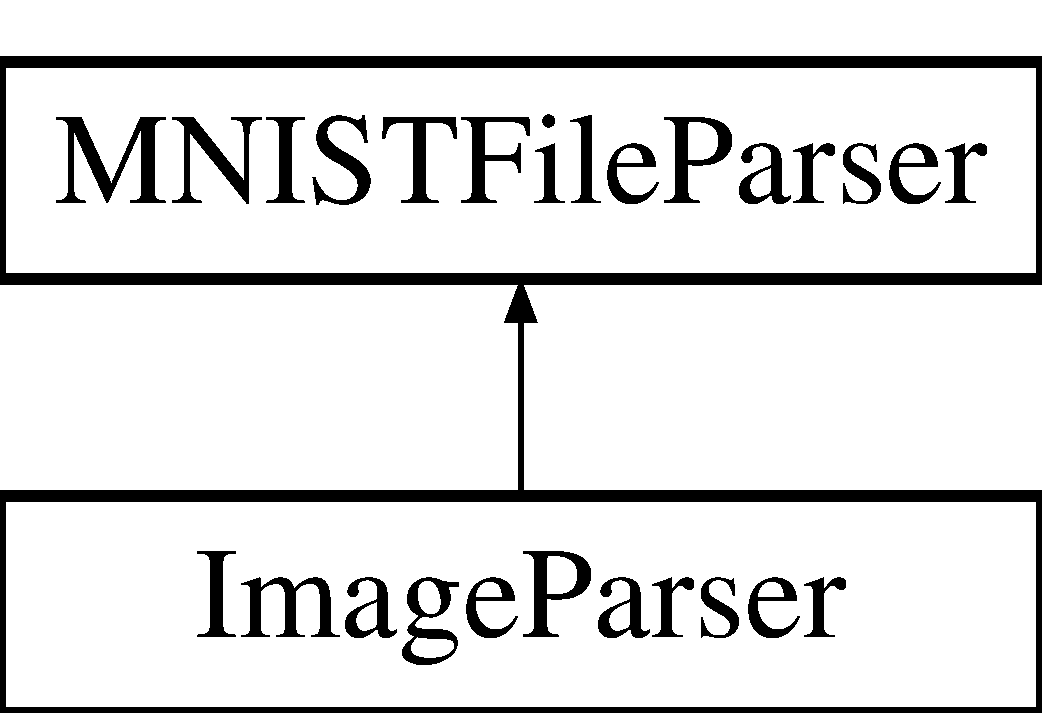
\includegraphics[height=2.000000cm]{class_image_parser}
\end{center}
\end{figure}
\subsection*{Public Member Functions}
\begin{DoxyCompactItemize}
\item 
\mbox{\Hypertarget{class_image_parser_a5e392f9752e88ebcec8e2d2d2334d31e}\label{class_image_parser_a5e392f9752e88ebcec8e2d2d2334d31e}} 
{\bfseries Image\+Parser} (std\+::string filename)
\item 
\mbox{\Hypertarget{class_image_parser_ad4e5313519b0ee20b30ffb64b2b9c736}\label{class_image_parser_ad4e5313519b0ee20b30ffb64b2b9c736}} 
virtual void {\bfseries parse} ()
\end{DoxyCompactItemize}
\subsection*{Additional Inherited Members}


The documentation for this class was generated from the following files\+:\begin{DoxyCompactItemize}
\item 
C\+:/\+Users/charc/source/repos/ff\+Neural\+Net/\+Neural\+Net/M\+N\+I\+S\+T\+File\+Parser.\+h\item 
C\+:/\+Users/charc/source/repos/ff\+Neural\+Net/\+Neural\+Net/M\+N\+I\+S\+T\+File\+Parser.\+cpp\end{DoxyCompactItemize}

\hypertarget{class_label_parser}{}\section{Label\+Parser Class Reference}
\label{class_label_parser}\index{Label\+Parser@{Label\+Parser}}
Inheritance diagram for Label\+Parser\+:\begin{figure}[H]
\begin{center}
\leavevmode
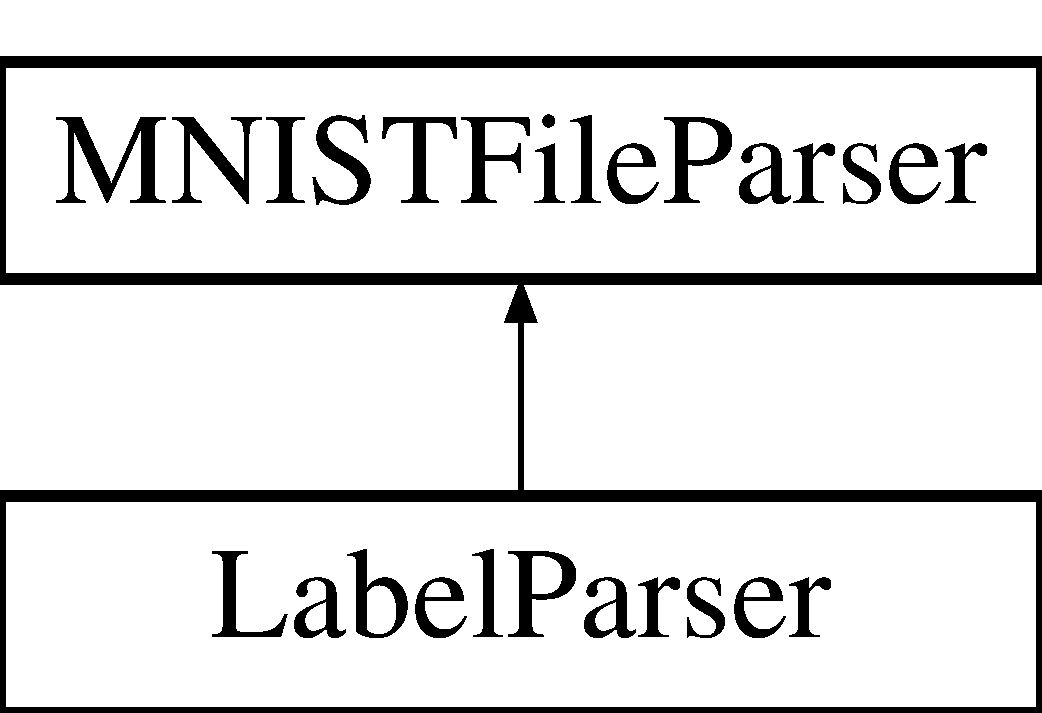
\includegraphics[height=2.000000cm]{class_label_parser}
\end{center}
\end{figure}
\subsection*{Public Member Functions}
\begin{DoxyCompactItemize}
\item 
\mbox{\Hypertarget{class_label_parser_a42e1312b018e61d541562197b304c31a}\label{class_label_parser_a42e1312b018e61d541562197b304c31a}} 
{\bfseries Label\+Parser} (std\+::string filename)
\item 
\mbox{\Hypertarget{class_label_parser_af8bd2f907738f36487f7220ec792fc43}\label{class_label_parser_af8bd2f907738f36487f7220ec792fc43}} 
virtual void {\bfseries parse} ()
\end{DoxyCompactItemize}
\subsection*{Additional Inherited Members}


The documentation for this class was generated from the following files\+:\begin{DoxyCompactItemize}
\item 
C\+:/\+Users/charc/source/repos/ff\+Neural\+Net/\+Neural\+Net/M\+N\+I\+S\+T\+File\+Parser.\+h\item 
C\+:/\+Users/charc/source/repos/ff\+Neural\+Net/\+Neural\+Net/M\+N\+I\+S\+T\+File\+Parser.\+cpp\end{DoxyCompactItemize}

\hypertarget{class_m_n_i_s_t_file_parser}{}\section{M\+N\+I\+S\+T\+File\+Parser Class Reference}
\label{class_m_n_i_s_t_file_parser}\index{M\+N\+I\+S\+T\+File\+Parser@{M\+N\+I\+S\+T\+File\+Parser}}
Inheritance diagram for M\+N\+I\+S\+T\+File\+Parser\+:\begin{figure}[H]
\begin{center}
\leavevmode
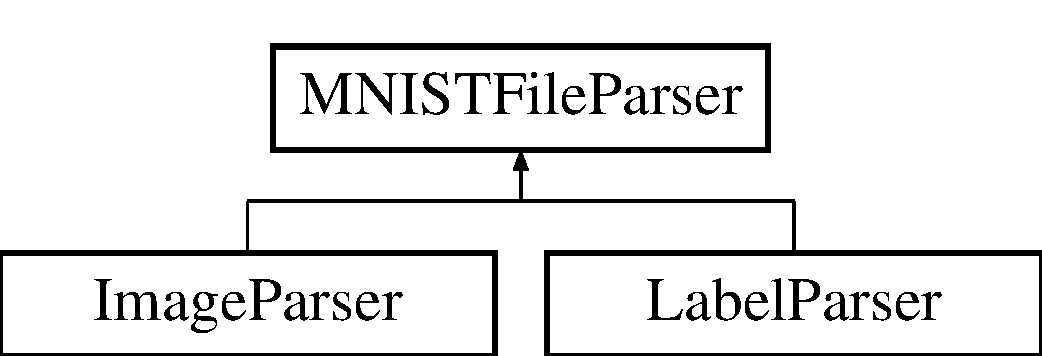
\includegraphics[height=2.000000cm]{class_m_n_i_s_t_file_parser}
\end{center}
\end{figure}
\subsection*{Public Member Functions}
\begin{DoxyCompactItemize}
\item 
\mbox{\Hypertarget{class_m_n_i_s_t_file_parser_a4e50774bc3ff914f91742020ebddd842}\label{class_m_n_i_s_t_file_parser_a4e50774bc3ff914f91742020ebddd842}} 
{\bfseries M\+N\+I\+S\+T\+File\+Parser} (std\+::string filename)
\item 
\mbox{\Hypertarget{class_m_n_i_s_t_file_parser_a77153a0159347e41761c0948b34a8893}\label{class_m_n_i_s_t_file_parser_a77153a0159347e41761c0948b34a8893}} 
virtual void {\bfseries parse} (void)=0
\item 
\mbox{\Hypertarget{class_m_n_i_s_t_file_parser_a91934edbf3852030ef9341281491637e}\label{class_m_n_i_s_t_file_parser_a91934edbf3852030ef9341281491637e}} 
Eigen\+::\+Matrix\+Xd $\ast$ {\bfseries get\+Data} (void) const
\item 
\mbox{\Hypertarget{class_m_n_i_s_t_file_parser_afd1183b4334e41d9e5060e70c07b5759}\label{class_m_n_i_s_t_file_parser_afd1183b4334e41d9e5060e70c07b5759}} 
std\+::pair$<$ int, int $>$ {\bfseries data\+Size} (void) const
\item 
\mbox{\Hypertarget{class_m_n_i_s_t_file_parser_a2cc71c0f1ada30d6039f1f90d864696d}\label{class_m_n_i_s_t_file_parser_a2cc71c0f1ada30d6039f1f90d864696d}} 
void {\bfseries set\+Record\+Cap} (int cap)
\item 
\mbox{\Hypertarget{class_m_n_i_s_t_file_parser_ab01a79cb739cb2e90226240365e11f30}\label{class_m_n_i_s_t_file_parser_ab01a79cb739cb2e90226240365e11f30}} 
int {\bfseries get\+Num\+Records} (void) const
\end{DoxyCompactItemize}
\subsection*{Protected Attributes}
\begin{DoxyCompactItemize}
\item 
\mbox{\Hypertarget{class_m_n_i_s_t_file_parser_a40515ef5800bb10620ab6cac6c994750}\label{class_m_n_i_s_t_file_parser_a40515ef5800bb10620ab6cac6c994750}} 
const std\+::string {\bfseries filename}
\item 
\mbox{\Hypertarget{class_m_n_i_s_t_file_parser_a658bfcf8d881bc2a6c9e73ae13be7fa4}\label{class_m_n_i_s_t_file_parser_a658bfcf8d881bc2a6c9e73ae13be7fa4}} 
int {\bfseries magic\+\_\+number}
\item 
\mbox{\Hypertarget{class_m_n_i_s_t_file_parser_a2d6456b4f107c05afd748ad5ae5dfda3}\label{class_m_n_i_s_t_file_parser_a2d6456b4f107c05afd748ad5ae5dfda3}} 
int {\bfseries num\+\_\+records}
\item 
\mbox{\Hypertarget{class_m_n_i_s_t_file_parser_aa51099df794558d800bc45952a96b072}\label{class_m_n_i_s_t_file_parser_aa51099df794558d800bc45952a96b072}} 
Eigen\+::\+Matrix\+Xd $\ast$ {\bfseries data}
\item 
\mbox{\Hypertarget{class_m_n_i_s_t_file_parser_a6d7f525b818599dd33748e941453cdcc}\label{class_m_n_i_s_t_file_parser_a6d7f525b818599dd33748e941453cdcc}} 
std\+::ifstream {\bfseries fs}
\item 
\mbox{\Hypertarget{class_m_n_i_s_t_file_parser_a9dc6f336f0c71750f8118905edc23c47}\label{class_m_n_i_s_t_file_parser_a9dc6f336f0c71750f8118905edc23c47}} 
int {\bfseries record\+\_\+cap}
\end{DoxyCompactItemize}


The documentation for this class was generated from the following files\+:\begin{DoxyCompactItemize}
\item 
C\+:/\+Users/charc/source/repos/ff\+Neural\+Net/\+Neural\+Net/M\+N\+I\+S\+T\+File\+Parser.\+h\item 
C\+:/\+Users/charc/source/repos/ff\+Neural\+Net/\+Neural\+Net/M\+N\+I\+S\+T\+File\+Parser.\+cpp\end{DoxyCompactItemize}

%--- End generated contents ---

% Index
\backmatter
\newpage
\phantomsection
\clearemptydoublepage
\addcontentsline{toc}{chapter}{Index}
\printindex

\end{document}
